\chapter{Camera Calibration and Stereo Vision}
\noindent
Las cámaras fotográficas operan esencialmente como máquinas de reducción de dimensionalidad, proyectando el mundo tridimensional real $\mathbb{R}^3$ sobre un plano bidimensional discreto $\mathbb{R}^2$. El modelo matemático estándar que describe este fenómeno es la \tbf{Cámara Pinhole}. \\

\noindent
La relación geométrica exacta entre un punto del espacio tridimensional expresado en coordenadas homogéneas $\mathbf{X} = [X, Y, Z, 1]^T$ y su correspondiente proyección en el plano de la imagen en píxeles homogéneos $\mathbf{x} = [x_h, y_h, w]^T$ se define mediante la \tbf{Ecuación Proyectiva de la Cámara}:

$$\mathbf{x} \sim P\mathbf{X}$$
donde $P$ es la \tbf{Matriz de la Cámara (Camera Matrix)}, una matriz de dimensiones $3 \times 4$ y con 11 grados de libertad independientes que concentra tanto la geometría interna como la posición espacial del dispositivo. \\

\noindent
Para entender las matrices, primero debemos saber que el ordenador maneja tres ``mundos'' o sistemas de referencia:
\begin{itemize}
    \item \textbf{Mundo Real ($\mathbf{X}_w$):} donde las coordenadas se miden en metros respecto a un origen arbitrario (ej. la esquina de la habitación).
    \item \textbf{Cámara ($\mathbf{X}_c$):} un sistema donde el origen $(0,0,0)$ es exactamente el centro óptico (el "ojo") de la cámara. El eje $Z$ apunta hacia adelante (eje óptico), el eje $X$ a la derecha y el eje $Y$ hacia abajo.
    \item \textbf{Imagen ($\mathbf{x}$):} el plano 2D digital medido puramente en píxeles.
\end{itemize}

\section{Descomposición de la Matriz de la Cámara $P$}
La matriz global de proyección $P$ se puede descomponer algebraicamente en el producto de dos bloques de matrices diferenciados, mapeando el punto desde el sistema global del universo, pasando por el ojo de la cámara, hasta el sensor digital:

$$P = K \, [R \mid \mathbf{t}]$$
donde $K$ contiene los parámetros intrínsecos de la cámara (de tamaño $3 \times 3$) y $[R \mid \mathbf{t}]$ representa los parámetros extrínsecos (de tamaño $3 \times 4$).

\subsection{Parámetros Intrínsecos (Matriz $K$)}
\noindent
Los \tbf{parámetros intrínsecos} describen las propiedades geométricas y ópticas internas de la cámara. Su calibración es fija e independiente de dónde se coloque el dispositivo en el espacio. La matriz $K$ se estructura de la siguiente forma:

$$K = \begin{bmatrix} f_x & s & c_x \\ 0 & f_y & c_y \\ 0 & 0 & 1 \end{bmatrix}$$

\begin{itemize}
    \item \textbf{Distancia Focal ($f_x, f_y$):} Representa la distancia desde el centro óptico (pinhole) hasta el plano del sensor, expresada en unidades de píxeles en lugar de metros o milímetros para absorber el tamaño físico de los fotosentidos en los ejes $X$ e $Y$. \\
    
    \noindent
    En una cámara cualquier, el sensor del foco de una camara es donde se recoge la información de luz, mientras que el pinhole es el punto de proyección, que nosotros lo pensaremos como la lente de cristal por el que entra toda la información (lo que viene a ser el cristal que podemos limpiar). La distancia focal es la distancia entre el pinhole y el sensor, y es un parámetro fundamental que determina el campo de visión de la cámara, y es propio de esta. Aunque de primeras pensemos que tiene sentido que se mida dicha distancia en milímetros, se mide en pixeles porque el tamaño físico del sensor (y por tanto el tamaño de cada píxel) varía entre cámaras.
    \item \textbf{Punto Principal ($c_x, c_y$):} son las coordenadas del centro óptico de proyección, \tbf{pinhole} (el eje óptico que intersecta perpendicularmente al sensor) medidas en el sistema de píxeles de la imagen (típicamente cercano al centro de la resolución de la foto). Es el punto exacto donde la luz se concentra y se cruza.
    \item \textbf{Factor de Cizalladura / Skew ($s$):} mide la falta de ortogonalidad o la distorsión angular entre los ejes de píxeles del sensor. En las cámaras modernas, este valor es prácticamente cero ($s = 0$).
\end{itemize}

\subsection{Parámetros Extrínsecos ($[R \mid \mathbf{t}]$)}
\noindent
Los \tbf{parámetros extrínsecos} definen la transformación de cuerpo rígido que mapea las coordenadas desde el sistema de referencia global del mundo real al sistema de coordenadas local de la cámara:
\begin{itemize}
    \item \textbf{Matriz de Rotación ($R$):} una matriz ortogonal de $3 \times 3$ ($R^T R = I$ que implica que no deforma el espacio) con 3 grados de libertad (que corresponden a los tres giros posibles en el espacio tridimensional) que orienta los ejes de la cámara respecto al universo. El objetivo es alinear los ejes de coordenadas del mundo con los ejes de la cámara, es decir, se encarga de girar los ejes del espacio para que el eje $X$ de la habitación mire hacia el mismo lado que el eje $X$ de la cámara, y lo mismo con el $Y$ y el $Z$. Los tres movimientos básicos son
    \begin{itemize}
        \item \tbf{Pan (o Yaw)}: girar la cámara hacia la izquierda o la derecha.
        \item \tbf{Tilt (o Pitch)}: cabecear la cámara hacia arriba o hacia abajo.
        \item \tbf{Roll}: inclinar la cámara de lado (como cuando ladeas la cabeza para poner una foto en vertical).
    \end{itemize}
    
    \item \textbf{Vector de Traslación ($\mathbf{t}$):} un vector de $3 \times 1$ que desplaza el origen de coordenadas global hasta la posición física del centro óptico de la cámara, dado como sigue
    $$\mathbf{t} = \begin{bmatrix} t_x \\ t_y \\ t_z \end{bmatrix}$$
    El vector $\mathbf{t}$ mide simplemente el desplazamiento físico en el espacio entre los dos orígenes de coordenadas. Te dice cuántos metros tienes que caminar desde el origen de coordenadas del mundo hasta llegar al centro del objetivo de la cámara (origen de la cámara).
\end{itemize}

\section{Algoritmo de Calibración de la Cámara}
El objetivo del \tbf{Algoritmo de Calibración} es estimar numéricamente de forma precisa los elementos de la matriz intrínseca $K$ y los parámetros extrínsecos $[R \mid \mathbf{t}]$. El algoritmo es un método de estimación pasivo: requiere que le demos datos de entrada conocidos.

\begin{enumerate}
    \item \textbf{Inputs de Calibración (Calibración Pasiva):} se colocan imágenes de un patrón de geometría perfectamente conocida de distintos ángulos, comúnmente una \underline{plantilla de tablero de} \underline{ajedrez (checkerboard images)}, donde se conocen exactamente las coordenadas 3D de cada esquina del tablero en el sistema de referencia del mundo.
    \item \textbf{Correspondencias de Puntos:} para cada una de las imágenes capturadas, el algoritmo debe identificar un conjunto de $n$ puntos de control.
    \begin{itemize}
        \item Definimos un sistema de coordenadas del mundo virtual fijando el origen $(0,0,0)_w$ en la esquina superior izquierda del tablero físico. Cada esquina del tablero tiene coordenadas métricas 3D conocidas en este sistema, por ejemplo: $\mathbf{X}_w^{(1)} = (0, 0, 0)^T$, $\mathbf{X}_w^{(2)} = (30, 0, 0)^T$ (en milímetros). Podemos calcular de forma exacta y perfecta la posición tridimensional de cada esquina interna en el plano del tablero ($Z_w=0$)
        $$\mathbf{X}_w^{(1)} = (0, 0, 0)^T, \quad \mathbf{X}_w^{(2)} = (30, 0, 0)^T, \quad \mathbf{X}_w^{(3)} = (60, 0, 0)^T \dots$$
        \item El ordenador procesa la fotografía digital utilizando detectores de esquinas basados en gradientes de brillo (como el detector de Harris o algoritmos de análisis de sillas de montar). Localiza en qué coordenadas de píxeles exactas de la pantalla ha salido retratada cada una de esas esquinas
        $$\mathbf{u}^{(1)} = (u^{(1)}, v^{(1)})^T, \quad \mathbf{u}^{(2)} = (u^{(2)}, v^{(2)})^T \dots$$
       
        \item Al final de este paso, tenemos una lista de parejas $\left\{ \left(\mathbf{X}_w^{(i)}, \mathbf{u}^{(i)}\right) \right\}_{i=1}^{n}$ que correlacionan el espacio real con la foto.
    \end{itemize}

    \item \textbf{Estimación Matemática (DLT):} sabemos que la cámara proyecta los puntos siguiendo el modelo pinhole homogéneo $\mathbf{x} \sim P\mathbf{X}$, donde $P$ es la matriz de la cámara de tamaño $3 \times 4$ compuesta por 12 incógnitas ($p_{11}$ hasta $p_{34}$). Si expandimos la multiplicación de la matriz por el vector del mundo para un punto $i$, el sistema nos dicta
    
    $$\begin{bmatrix} w \cdot u^{(i)} \\ w \cdot v^{(i)} \\ w \end{bmatrix} = \begin{bmatrix} p_{11} & p_{12} & p_{13} & p_{14} \\ p_{21} & p_{22} & p_{23} & p_{24} \\ p_{31} & p_{32} & p_{33} & p_{34} \end{bmatrix} \begin{bmatrix} X_w^{(i)} \\ Y_w^{(i)} \\ Z_w^{(i)} \\ 1 \end{bmatrix}$$
    Para deshacernos del factor de escala ``fantasma'' $w$, sustituimos la tercera fila ($w = p_{31}X_w^{(i)} + p_{32}Y_w^{(i)} + p_{33}Z_w^{(i)} + p_{34}$) en las dos primeras filas. Al hacer esto, obtenemos las ecuaciones no lineales de proyección real en píxeles
        
        $$u^{(i)} = \frac{p_{11}X_w^{(i)} + p_{12}Y_w^{(i)} + p_{13}Z_w^{(i)} + p_{14}}{p_{31}X_w^{(i)} + p_{32}Y_w^{(i)} + p_{33}Z_w^{(i)} + p_{34}} \quad , \quad v^{(i)} = \frac{p_{21}X_w^{(i)} + p_{22}Y_w^{(i)} + p_{23}Z_w^{(i)} + p_{24}}{p_{31}X_w^{(i)} + p_{32}Y_w^{(i)} + p_{33}Z_w^{(i)} + p_{34}}$$
    
    \item \tbf{Rearrange into a linear system:} para procesar todos los puntos a la vez, el ordenador vectoriza los 12 elementos desconocidos de la matriz en un único vector columna largo $\mathbf{p} = (p_{11}, p_{12}, \dots, p_{34})^T$ de tamaño $12 \times 1$. Al apilar las filas de coeficientes conocidos (compuestos por las coordenadas físicas y los píxeles medidos), construimos una matriz gigante $A$ de tamaño $2n \times 12$, es decir, para cada punto tenemos estas dos ecuaciones
    \begin{align*}
        p_{11}X_w^{(i)} + p_{12}Y_w^{(i)} + p_{13}Z_w^{(i)} + p_{14} - u^{(i)}X_w^{(i)}p_{31} - u^{(i)}Y_w^{(i)}p_{32} - u^{(i)}Z_w^{(i)}p_{33} - u^{(i)}p_{34} =& 0 \\
        p_{21}X_w^{(i)} + p_{22}Y_w^{(i)} + p_{23}Z_w^{(i)} + p_{24} - v^{(i)}X_w^{(i)}p_{31} - v^{(i)}Y_w^{(i)}p_{32} - v^{(i)}Z_w^{(i)}p_{33} - v^{(i)}p_{34} =& 0 
    \end{align*}
    que equivale en forma matricial a
    \begin{equation*}
        \left[
        \begin{array}{cccccccccccc} 
            X_w^{(i)} & Y_w^{(i)} & Z_w^{(i)} & 1 & 0 & 0 & 0 & 0 & -u^{(i)}X_w^{(i)} & -u^{(i)}Y_w^{(i)} & -u^{(i)}Z_w^{(i)} & -u^{(i)} \\ 
            0 & 0 & 0 & 0 & X_w^{(i)} & Y_w^{(i)} & Z_w^{(i)} & 1 & -v^{(i)}X_w^{(i)} & -v^{(i)}Y_w^{(i)} & -v^{(i)}Z_w^{(i)} & -v^{(i)} 
        \end{array}
        \right]
        \begin{bmatrix} 
            p_{11} \\ p_{12} \\ p_{13} \\ p_{14} \\ p_{21} \\ p_{22} \\ p_{23} \\ p_{24} \\ p_{31} \\ p_{32} \\ p_{33} \\ p_{34} 
        \end{bmatrix} = 
        \begin{bmatrix} 
            0 \\ 0 
        \end{bmatrix}
    \end{equation*}
    de manera que el problema se reduce a resolver el siguiente sistema homogéneo
    $$\mathbf{A\mathbf{p} = \mathbf{0}}$$
    de dimensión $2n\times 12$.
    \item \tbf{Solve via SVD}: el sistema homogéneo $A\mathbf{p} = \mathbf{0}$ tiene una solución trivial $\mathbf{p} = \mathbf{0}$, que no es útil. Para encontrar la solución no trivial se busca minimizar el error de proyección (debido al ruido no conseguiremos esa igualdad exacta de $0$), es decir
    $$\|A\mathbf{p}\|^2$$
    donde restringiremos $\|p\|=1$ pues existen muchas matrices escalares de $P$ que representan la misma cámara. Para ellos se aplica la \tbf{Descomposición en Valores Singulares (SVD)} a la matriz $A$. \\
    
    \noindent
    La solución óptima es el vector singular de 
    $$A^T A$$
    correspondiente al valor singular más pequeño $\lambda_{\min}$ de $A$, que es equivalente al último vector de la matriz $V$ de la SVD de $A$, donde tenemos  
    $$A = U \Sigma V^T$$
\end{enumerate}

\begin{observacion}
    Dado $n \geq 6$ correspondencias 3D-2D, construimos la matriz $A$ de tamaño $2n \times 12$, calculamos la SVD de $A$ y tomamos la última columna de $V$ como el vectorizado de la matriz de proyección $p$. Reshapeamos $p$ en la matriz de proyección $P$ de tamaño $3 \times 4$. Este procedimiento se llama el \tbf{Direct Linear Transform (DLT)}.
\end{observacion}

\subsection{Extracción de parámetros}
\noindent
Dada la matriz $P$ obtenida por el algoritmo de calibración, el siguiente paso es extraer los parámetros intrínsecos $K$ y extrínsecos $[R \mid \mathbf{t}]$ de forma separada, donde tenemos
\begin{equation*}
P = K \, [R \mid \mathbf{t}] = \begin{bmatrix} KR & \mid & K\mathbf{t} \end{bmatrix}
\end{equation*}

\begin{description}
    \item[Separar $K$ y $R$.] The left $3 \times 3$ sub-matrix of $P$ is the product $KR$
    \begin{equation*}
        \begin{bmatrix} p_{11} & p_{12} & p_{13} \\ p_{21} & p_{22} & p_{23} \\ p_{31} & p_{32} & p_{33} \end{bmatrix} = KR
    \end{equation*}
    since $K$ is upper-triangular and $R$ is orthonormal, their product can be uniquely decomposed using RQ factorisation (a variant of QR factorisation). This gives $K$ and $R$ separately.
    \item[Recovering the Translation $\mathbf{t}$.] The last column of the matrix $P$ is by definition the block $K\mathbf{t}$:
    \begin{equation*}
        \begin{bmatrix} p_{14} \\ p_{24} \\ p_{34} \end{bmatrix} = K\mathbf{t} \implies \mathbf{t} = K^{-1} \begin{bmatrix} p_{14} \\ p_{24} \\ p_{34} \end{bmatrix}
    \end{equation*}
    the camera centre in world coordinates can then be recovered as $\mathbf{c}_w = -R^T \mathbf{t}$.
\end{description}

\section{Stereo Vision Basics}
La visión estéreo emula la percepción tridimensional humana utilizando **dos cámaras o vistas separadas** horizontalmente por una distancia conocida para recuperar la tercera dimensión (la profundidad $Z$) ausente en una sola proyección plana.

\subsection{La Relación Disparidad-Profundidad}
\begin{definicion}
    Se define la \tbf{disparidad} ($d$) como la diferencia en la posición horizontal en píxeles que sufre la proyección de un mismo punto del espacio entre la imagen izquierda ($x_l$) y la imagen derecha ($x_r$)
    $$d = x_l - x_r$$
\end{definicion}

\noindent
A partir de la semejanza de triángulos en una geometría de cámaras perfectamente idealizada y alineada, se deduce la \tbf{Ecuación Fundamental de la Visión Estéreo}:

$$\mathbf{Z = \frac{f \cdot B}{d}}$$
donde:
\begin{itemize}
    \item $Z$: distancia de profundidad del punto al plano de las cámaras.
    \item $f$: distancia focal del sistema óptico.
    \item $B$: \tbf{línea de base (Baseline)}, la distancia física de separación horizontal entre los centros ópticos de ambas cámaras.
    \item $d$: disparidad calculada.
\end{itemize}

\subsection{Disparidad Map}
\noindent
El resultado de procesar un par estéreo es un \tbf{mapa de disparidad (Disparidad Map)}, que se puede interpretar de forma directa como un mapa de relieve geométrico inverso gracias a su ley de proporcionalidad:

\begin{itemize}
    \item \textbf{Mayor Disparidad $\Longrightarrow$ Objeto Cercano:} Si un objeto está muy próximo a las lentes, su salto de píxeles horizontal entre la imagen izquierda y derecha será gigante.
    \item \textbf{Menor Disparidad $\Longrightarrow$ Objeto Lejano:} Si el objeto está situado en el fondo de la escena o cerca del infinito, sus proyecciones impactarán prácticamente en las mismas coordenadas en ambas pantallas ($d \to 0$), lo que implica matemáticamente que la profundidad tiende a infinito ($Z \to \infty$).
\end{itemize}


\section{Image Rectification}
\begin{definicion}
    Si tú ves un punto en la imagen izquierda, en el mundo real ese píxel podría ser un objeto cercano, o un objeto mediano, o una estrella en el infinito. Ese píxel representa un rayo de luz infinito que sale de la cámara. Visto desde la segunda cámara, ese rayo de luz se ve como una línea recta inclinada que cruza su pantalla. Esa es la \tbf{línea epipolar}. Buscar el punto homólogo significa buscar a lo largo de esa línea inclinada. \\
\end{definicion}

\noindent
En una configuración física real, es mecánicamente imposible colocar dos cámaras de forma que queden perfectamente paralelas y alineadas a nivel de micras de píxel (situación que suponíamos antes). \\
\noindent
Debido a este desalineamiento físico, si intentas buscar el mismo punto en ambas imágenes, la línea epipolar (el camino donde se esconde el punto hermano) saldrá inclinada y torcida en diagonal a través de la pantalla de la segunda cámara. Para encontrar el punto homólogo, tu algoritmo tendría que buscar haciendo un barrido en dos dimensiones (2D): recorriendo píxel por píxel en horizontal y en vertical a lo largo de esa diagonal. Esto es computacionalmente lentísimo ($O(N^2)$) y propenso a errores.\\


\noindent
Esto obliga a realizar una fase de software previa llamada \tbf{rectificación}, lo que viene a ser ``enderezar la perspectiva de las fotos'', no tocamos las cámaras físicas, lo que hacemos es corregir las fotografías digitalmente por software después de haber sido tomadas.

\begin{itemize}
    \item \textbf{En qué consiste conceptualmente:} el algoritmo toma los parámetros de calibración que calculamos previamente (con el tablero de ajedrez) y calcula dos homografías (transformaciones proyectivas planas), una para la imagen izquierda ($H_L$) y otra para la derecha ($H_R$). \\

    \noindent
    Conceptualmente, es como si el ordenador tomara las dos fotos reales, las estirara y las retorciera matemáticamente en el aire, y las proyectara sobre un lienzo virtual común que es perfectamente plano (coplanar) y paralelo a la línea que une las dos cámaras. Es una ``cirugía de perspectiva''.
    \item \textbf{Alineamiento de Líneas Epipolares:} su efecto inmediato es que las líneas epipolares se vuelven \tbf{paralelas} y se \tbf{alinean horizontalmente} con las filas de la imagen.
    \item \textbf{Simplificación del Emparejamiento (Matching):} sin rectificación, buscar un punto homólogo requiere explorar toda la imagen en dos dimensiones (un coste de búsqueda 2D de $\mathcal{O}(N^2)$). Tras la rectificación, el punto homólogo de un píxel situado en la fila $Y=45$ de la imagen izquierda está garantizado que vive estrictamente en **la misma fila $Y=45$ de la imagen derecha**. La búsqueda se colapsa a un problema lineal unidimensional (1D) a lo largo de la fila, acelerando drásticamente el cálculo en tiempo real.
\end{itemize}
\noindent
Podemos ver una representación visual de la rectificación en la Figura \ref{fig:rectification}. Destacar que aunque en la figura se vea que solo queda una imagen para las dos homologías, esto no es del todo cierto, realmetne se crean dos imágenes, una para cada homología y por tanto para cada cámara, pero en la figura se ha representado solo una de ellas para simplificar la visualización. De manera, que se pasa de una imagen a otra manteniendo el eje $Y$ constante, es decir, la rectificación no cambia la coordenada vertical de los píxeles, solo la horizontal. Esto es lo que permite que las líneas epipolares se alineen horizontalmente y se vuelvan paralelas.
\begin{figure}
    \centering
    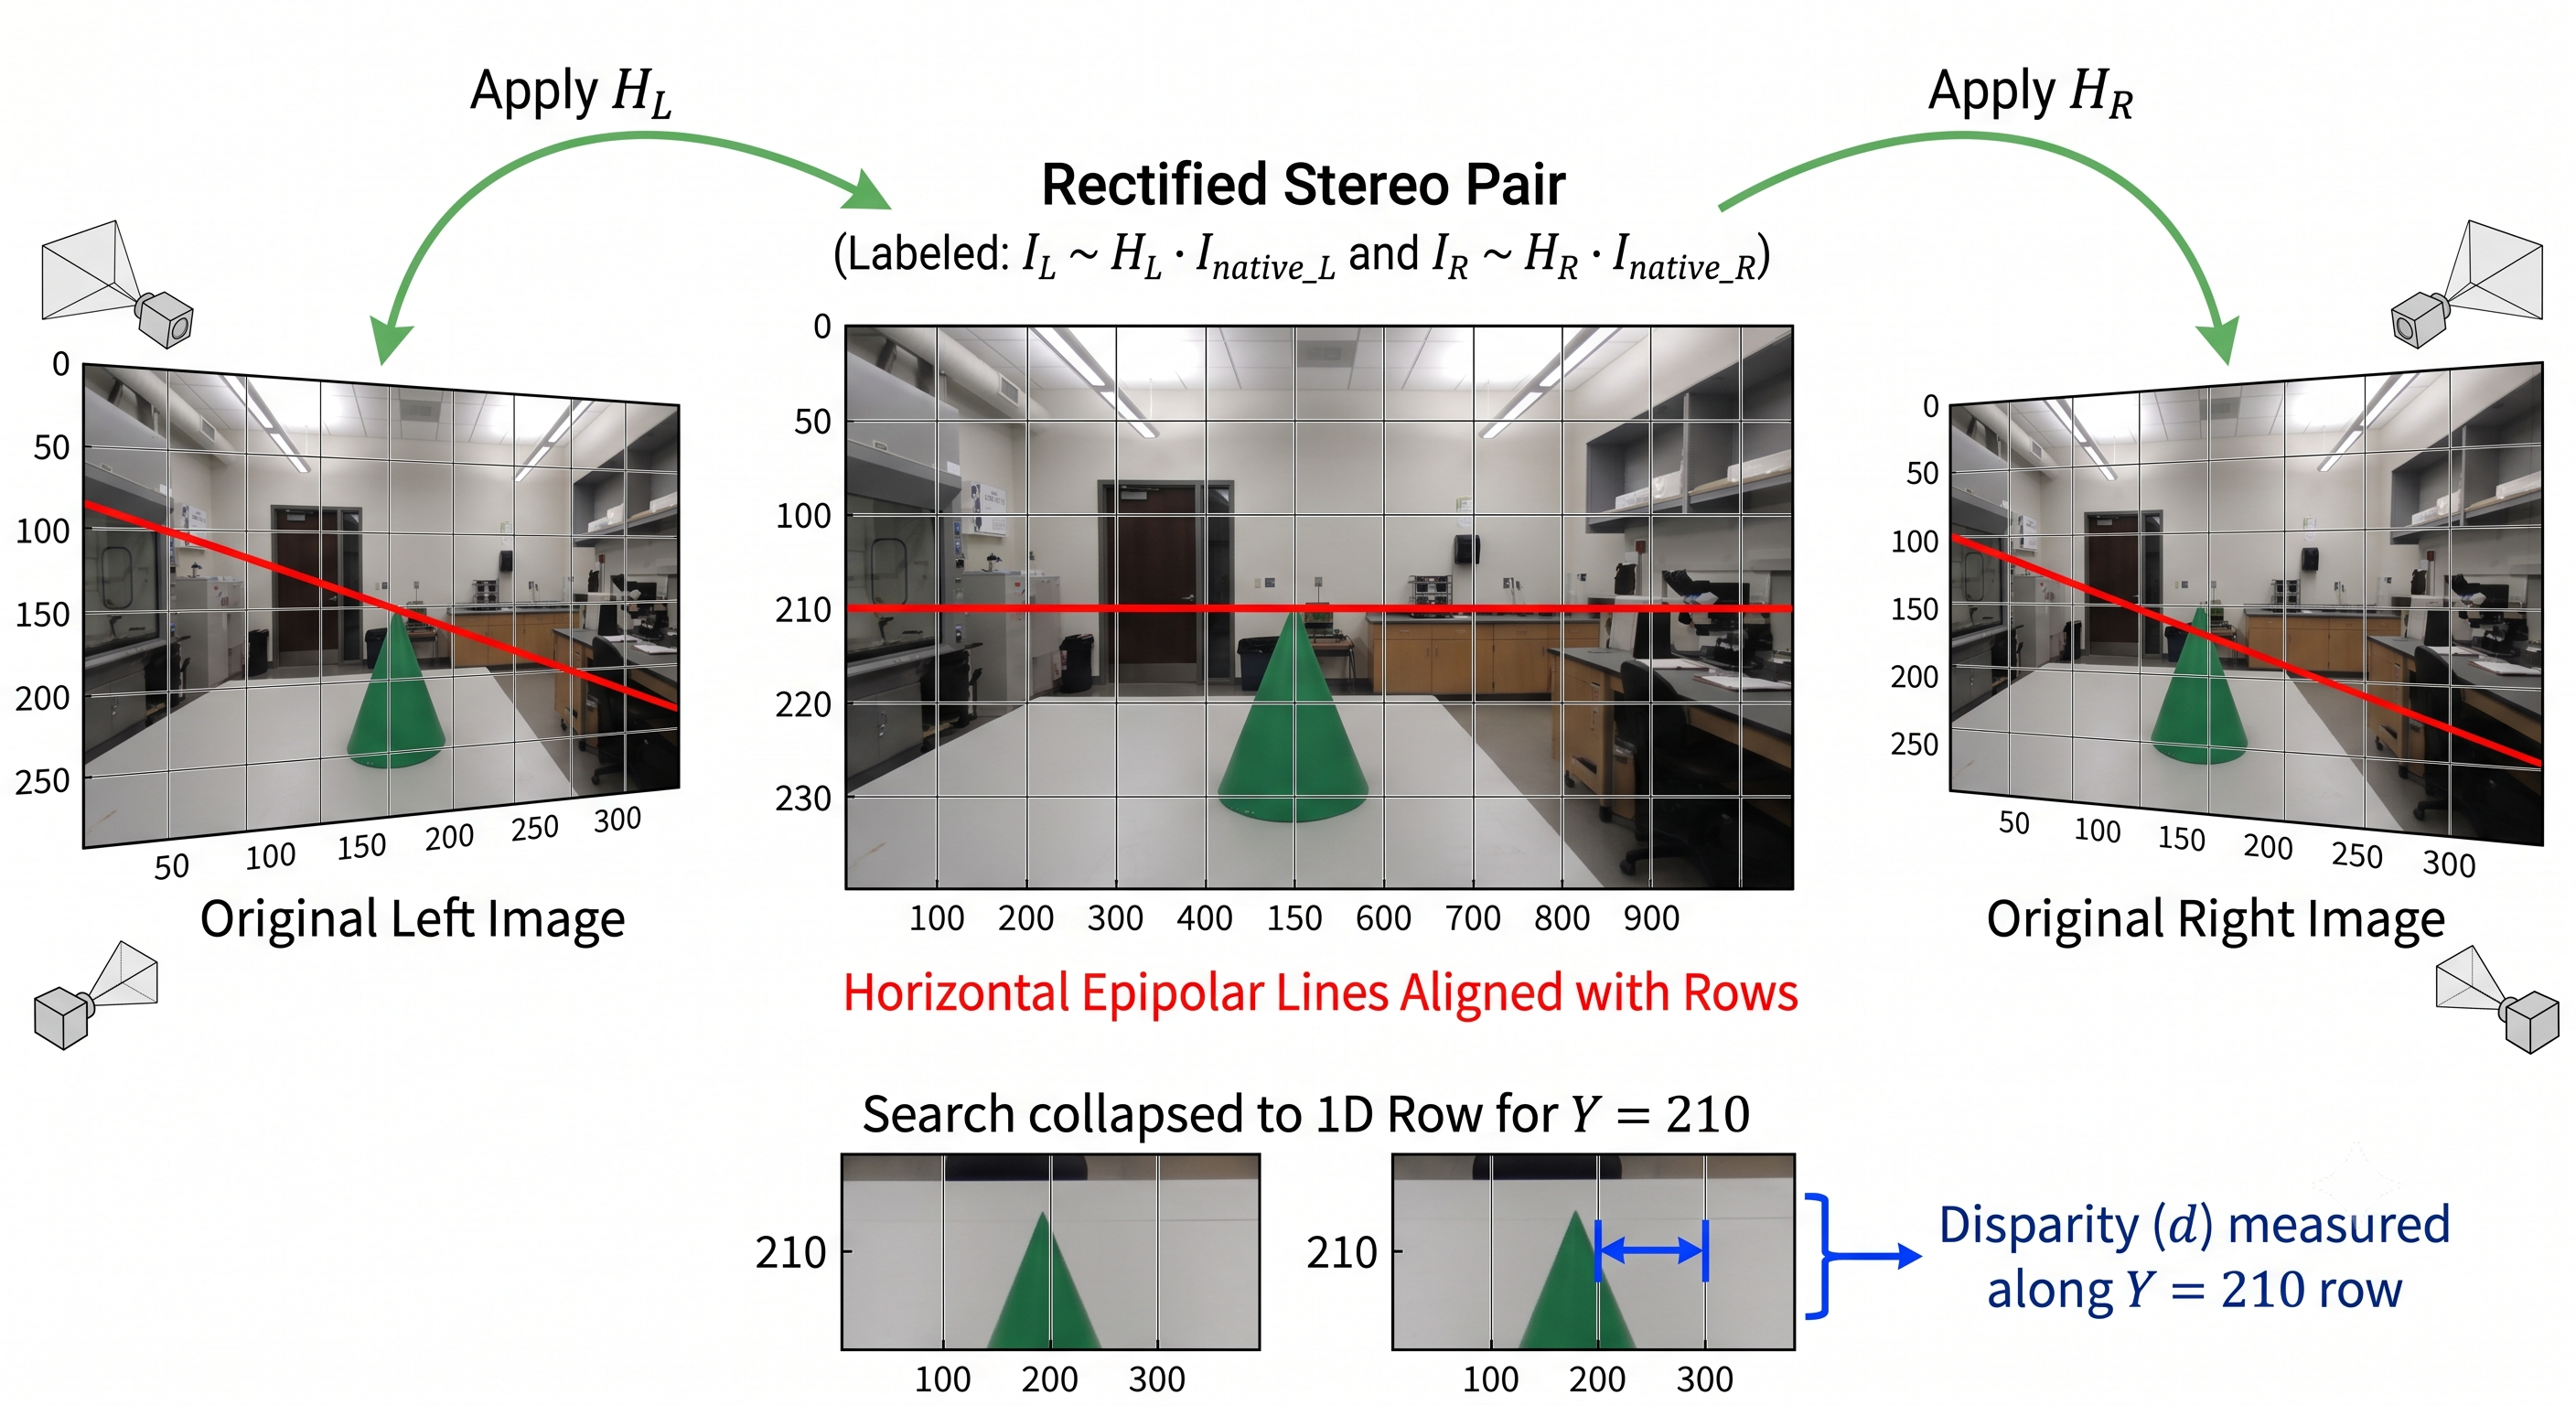
\includegraphics[width=0.8\textwidth]{img/rectification.png}
    \caption{Ejemplo de rectificación de la imagen.}
    \label{fig:rectification}
\end{figure}

